\documentclass[11pt,a4paper]{report}
\usepackage[portuges]{babel}
\usepackage[utf8]{inputenc} 
\usepackage{graphicx} 
\usepackage{url} 
\usepackage{enumerate} 
\usepackage{color} 
\usepackage{textcomp}
\usepackage{indentfirst}
\usepackage{array} 
\usepackage{parskip}
\usepackage[export]{adjustbox}
\usepackage{xpatch}
\newlength{\chaptertopskip}
\setlength{\chaptertopskip}{10pt}

\usepackage{a4wide}
\usepackage{float}
\usepackage{minted}
\usepackage{multicol}
\usepackage{appendix}
\setlength{\parskip}{1em}
\usepackage{verbatim}

\usepackage[demo]{graphicx}
\usepackage{caption}
\usepackage{subcaption}


\usepackage[pdftex]{hyperref} % transformar as referências internas do seu documento em hiper-ligações.

\definecolor{saddlebrown}{rgb}{0.55, 0.27, 0.07} % para definir uma nova cor, neste caso 'saddlebrown'

\usepackage{listings}  % para utilizar blocos de texto verbatim no estilo 'listings'
%paramerização mais vulgar dos blocos LISTING - GENERAL
\lstset{
	basicstyle=\small, %o tamanho das fontes que são usadas para o código
	numbers=left, % onde colocar a numeração da linha
	numberstyle=\tiny, %o tamanho das fontes que são usadas para a numeração da linha
	numbersep=5pt, %distancia entre a numeração da linha e o codigo
	breaklines=true, %define quebra automática de linha
    frame=tB,  % caixa a volta do codigo
	mathescape=true, %habilita o modo matemático
	escapeinside={(*@}{@*)} % se escrever isto  aceita tudo o que esta dentro das marcas e nao altera
}

\usepackage{xspace} % deteta se a seguir a palavra tem uma palavra ou um sinal de pontuaçao se tiver uma palavra da espaço, se for um sinal de pontuaçao nao da espaço

\parindent=20pt %espaço a deixar para fazer a  indentação da primeira linha após um parágrafo
\parskip=10pt % espaço entre o parágrafo e o texto anterior

\setlength{\oddsidemargin}{-1cm} %espaço entre o texto e a margem
\setlength{\textwidth}{18cm} %Comprimento do texto na pagina
\setlength{\headsep}{0cm} %espaço entre o texto e o cabeçalho
\setlength{\textheight}{23cm} %altura do texto na pagina
\renewcommand{\baselinestretch}{1.5cm}


\begin{document}
\begin{figure}
    
\includegraphics[scale=0.3]{logoum.png}
\end{figure}
\title{\textbf{Transformações Geométricas}\\
       \textbf{Unidade Curricular de Computação Gráfica}\\ Licenciatura em Ciências da Computação\\Universidade do Minho
       } %Titulo do documento
\author{Bruno Jardim\\ (A91680) \and Inês Presa\\ (A90355)
         \and Tiago Carriço\\ (A91695) \and Tiago Leite\\ (A91693)
       } %autores do documento
\date{\today} %data
\maketitle
\begingroup
\renewcommand*\contentsname{Índice}
\let\clearpage\relax
\tableofcontents


\endgroup
\newpage

\chapter{Contextualização}    
No âmbito da unidade curricular de Computação Gráfica da Licenciatura em Ciências da Computação foi proposta o desenvolvimento em \textit{Opengl} de um motor gráfico genérico que terá como função a criação de um sistema solar. Desenvolvimento esse que deve ser composto por quatro etapas. 

\section{Enunciado}
Nesta segunda etapa foi proposto:

\begin{itemize}
    \item \textbf{Cenas hierárquicas}
        \begin{description}
        \item Alteração do \textit{engine} de modo a ler ficheiros XML com vários grupos dispostos hierarquicamente. Um grupo pode ser composto por varias transformações geométricas(translação, rotação e escala), onde a ordem é relevante e opcionalmente por um ou mais modelos. 
        \end{description}

    \item \textbf{Ficheiro de configuração}
    \begin{description}
    \item Criação de um ficheiro de configuração XML que recrie um modelo estático do sistema solar, composto pelo sol, planetas, e luas dispostas hierarquicamente. 
    \end{description}
\end{itemize}


\chapter{Apresentação das soluções}
\section{Cenas hierárquicas}
Para a criação de cenas hierárquicas, procedeu-se à alteração do leitor XML desenvolvido na primeira fase. Assim sendo ao invés do que acontecia anteriormente de forma iterativa, agora o leitor trabalha de forma recursiva, numa de espécie de travessia em profundidade. Para tal, foi construída uma função auxiliar que recebe como argumentos qual o grupo a ler e um vetor com as transformações que vai herdar. Após a leitura de cada modelo, este é armazenado num vetor de modelos que é uma estrutura composta por um vetor de pontos, para desenhar a primitiva gráfica, e um vetor de transformações a aplicar antes da primitiva ser desenhada. De seguida, a função é chamada novamente recebendo como parametros o grupo descendente do atual e um vetor de transformações atualizado. Quando a função retorna do proceso recursivo para esta etapa, o processo é repetido para o grupo "irmão" do atual. \par
Para o a execução das transformaçoes foi criada uma classe abstracta chamada \textit{Transformation} com um metodo \textit{apply} e mais três outras classes, \textit{Translation}, \textit{Rotation},  e \textit{Scale} que implementam esta classe. Desta forma, para cada primitiva é possível iterar pelo vetor que armazena as transformações e simplesmente invocar o metodo \textit{apply}, não sendo por isso necessário executar instruções condicionais, como por exemplo \textit{if else}.  

\subsection{Demonstração do funcionamento do engine}

\vspace{1cm}
\begin{figure}[H]
\centering
\begin{subfigure}{0.5\textwidth}
  \centering
  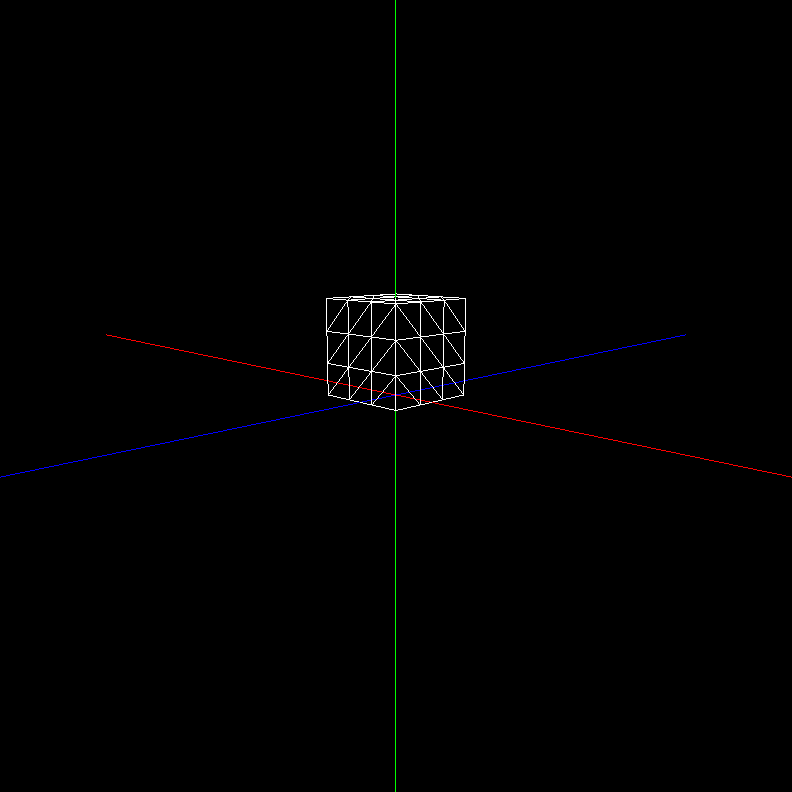
\includegraphics[width = 8cm,height = 8cm]{box.png}
  \caption{\texttt{test\_2\_1.xml}}
  \label{fig:box}
\end{subfigure}%
\begin{subfigure}{0.5\textwidth}
  \centering
  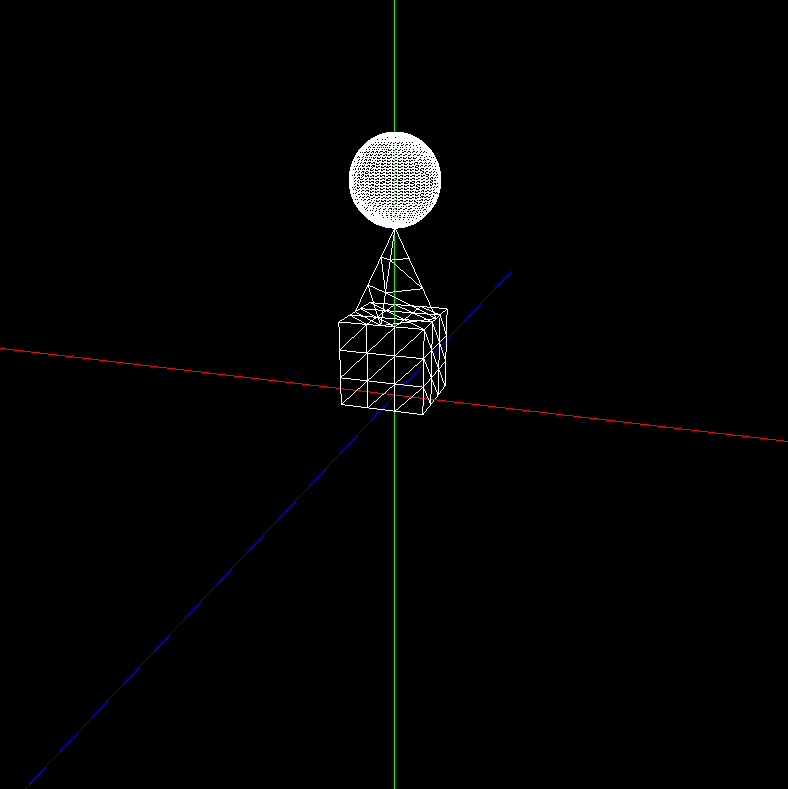
\includegraphics[width = 8cm,height = 8cm]{construction.png}
  \caption{\texttt{test\_2\_2.xml}}
  \label{fig:construction}
\end{subfigure}
\begin{subfigure}{0.5\textwidth}
  \centering
  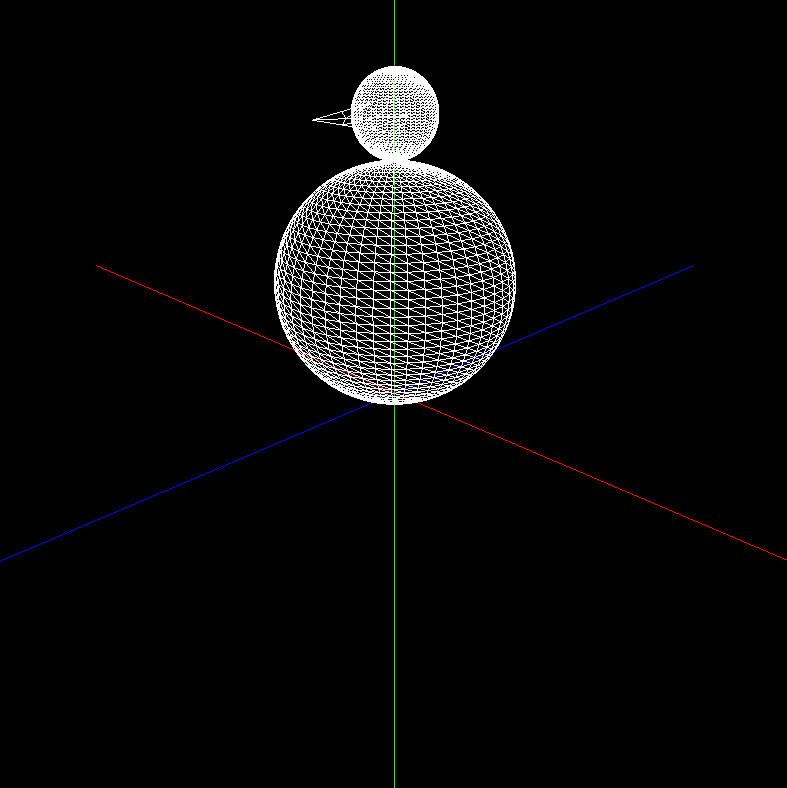
\includegraphics[width = 8cm,height = 8cm]{snowman.png}
  \caption{\texttt{test\_2\_3.xml}}
  \label{fig:snowman}
\end{subfigure}%
\begin{subfigure}{0.5\textwidth}
  \centering
  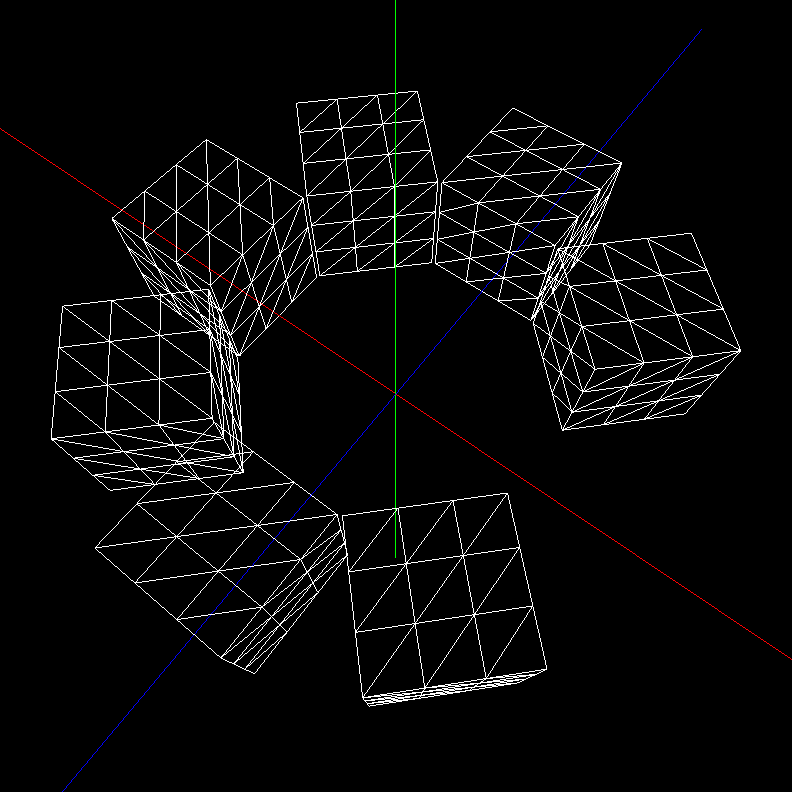
\includegraphics[width = 8cm,height = 8cm]{boxes.png}
  \caption{\texttt{test\_2\_4.xml}}
  \label{fig:sboxes}
\end{subfigure}
\label{fig:plano}
\caption{Execução dos ficheiros XML de teste}
\end{figure}
\textbf{Nota:} Nas imagens de teste apresentadas as esfera foram criadas com um número de stacks e slices superiores ao sugerido no ficheiro de configuração.


\newpage
\section{Ficheiro de configuração}
No ficheiro de configuração XML foi colocado o sol, os planetas e algumas das luas e anéis (conjuntos de luas) que orbitam os planetas. Para o calculo das distancias e tamanho dos planetas foi utilizado como medida de escala o diâmetro da Terra.

\vspace{1cm}
\begin{figure}[H]
\centering
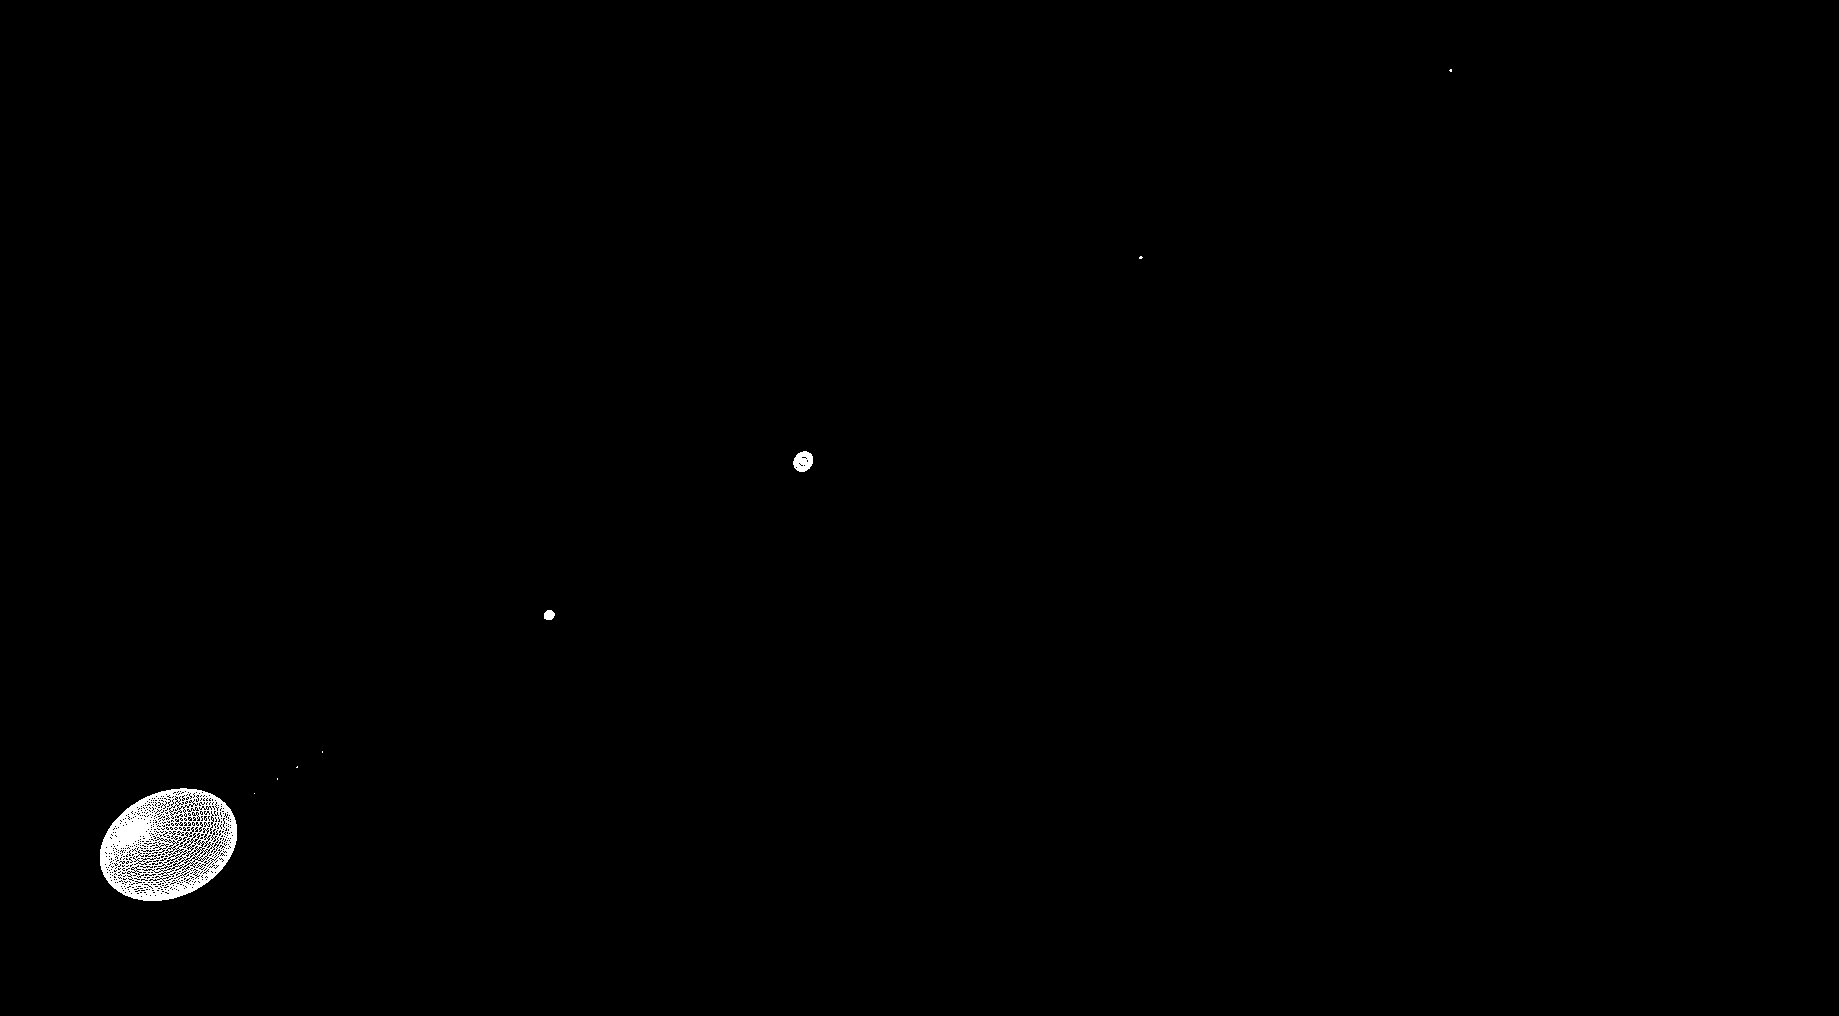
\includegraphics[width = 15cm,height = 10cm]{1.png}
\caption{\texttt{demo1}}
\label{fig:demo1}
\end{figure}

\begin{figure}[H]
\centering
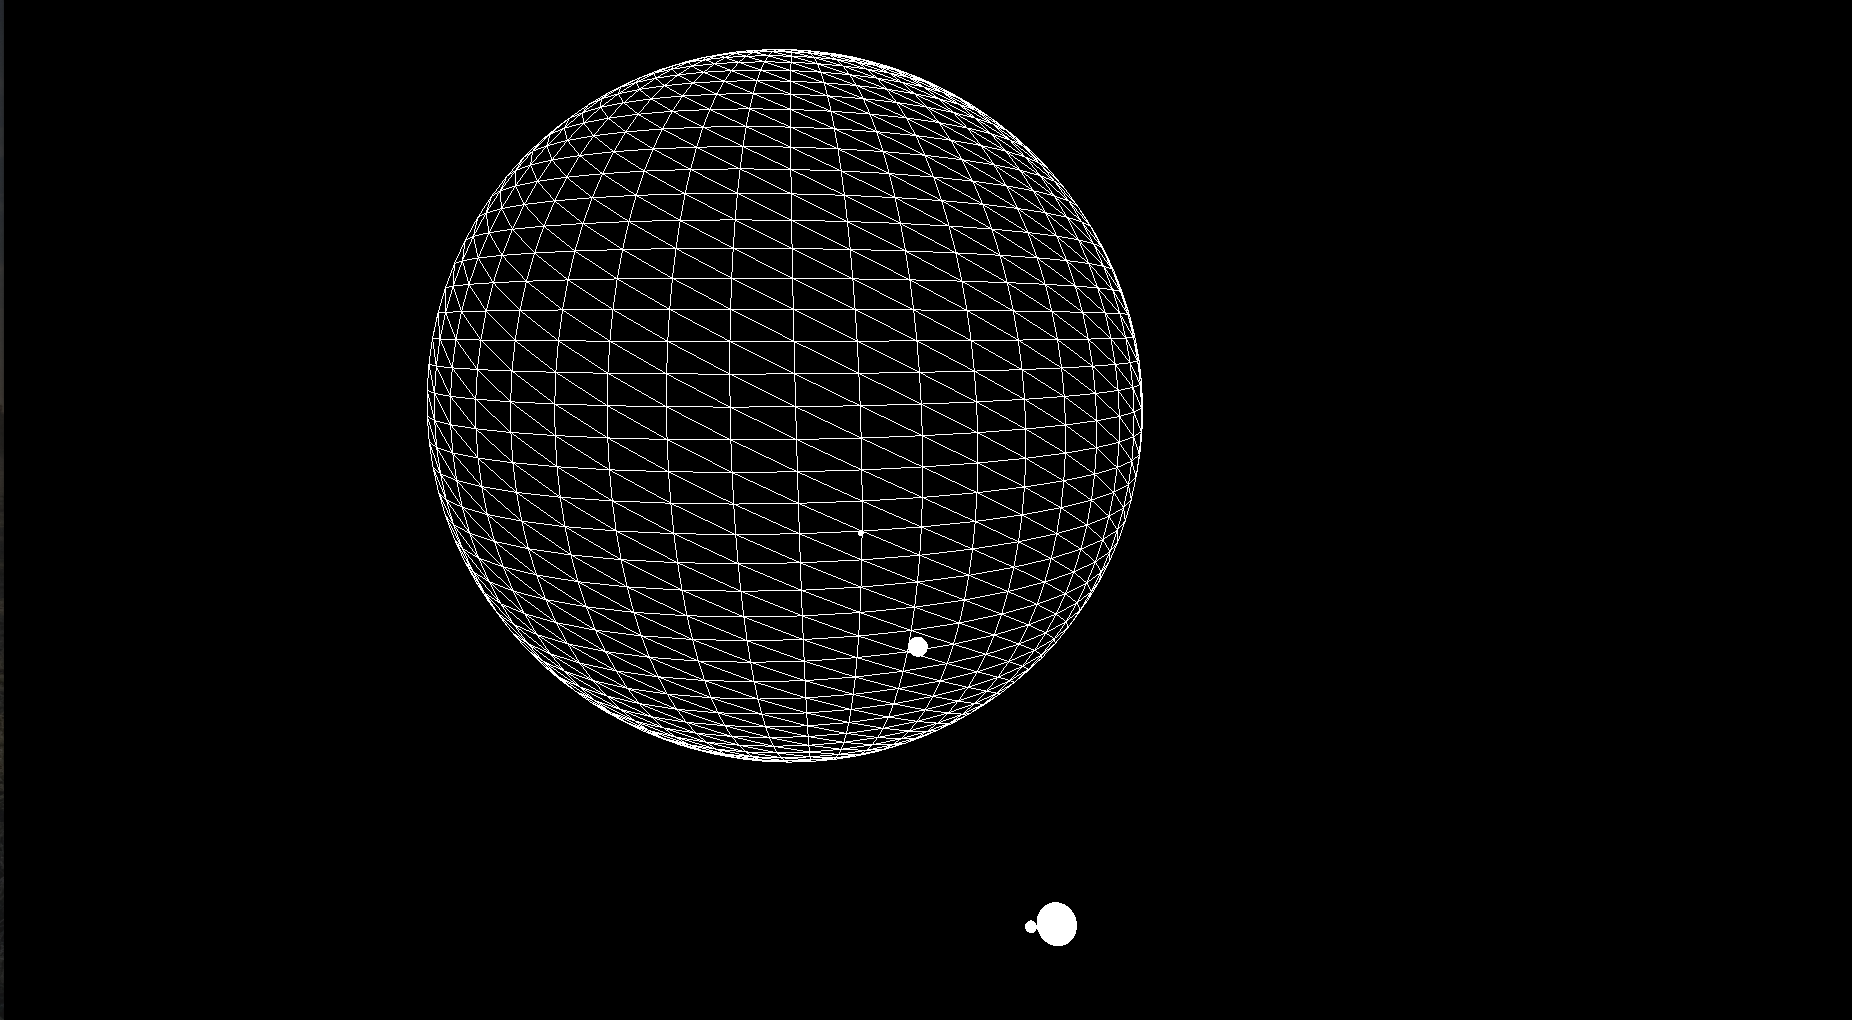
\includegraphics[width = 15cm,height = 10cm]{2.png}
\caption{\texttt{demo2}}
\label{fig:demo2}
\end{figure}

\begin{figure}[H]
\centering
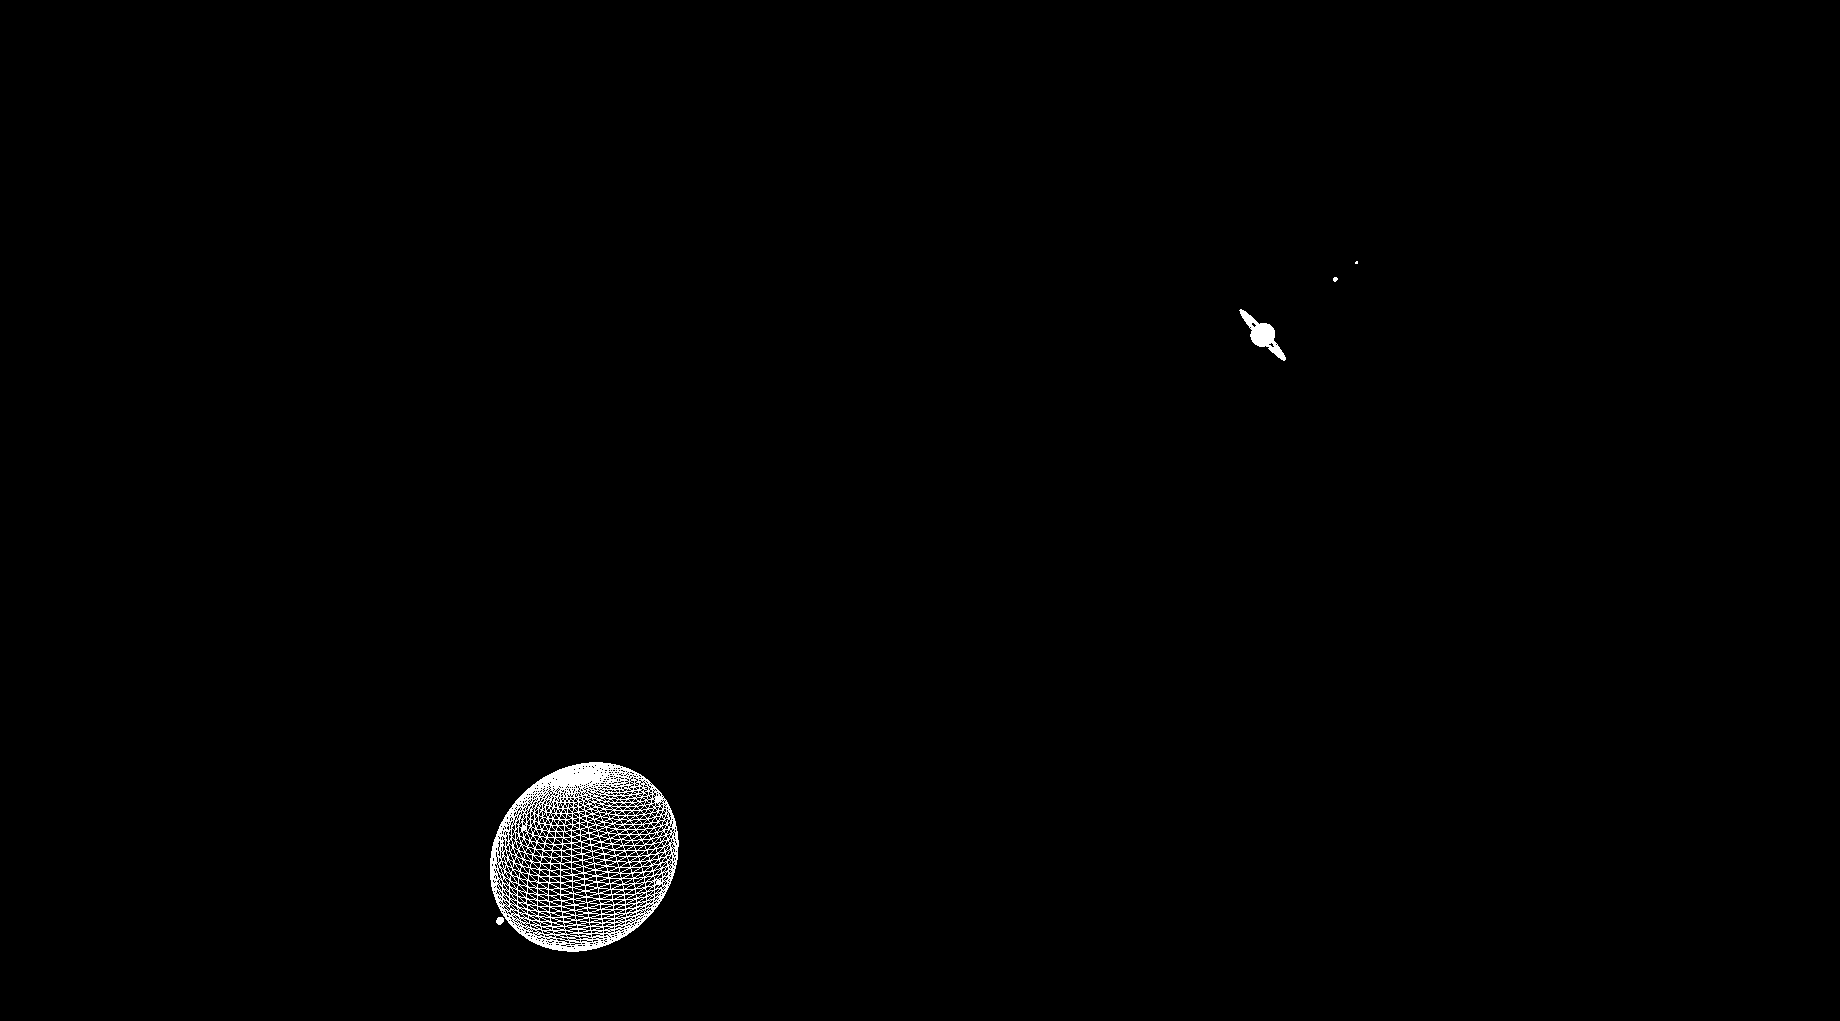
\includegraphics[width = 15cm,height = 10cm]{3.png}
\caption{\texttt{demo3}}
\label{fig:demo3}
\end{figure}

\begin{figure}[H]
\centering
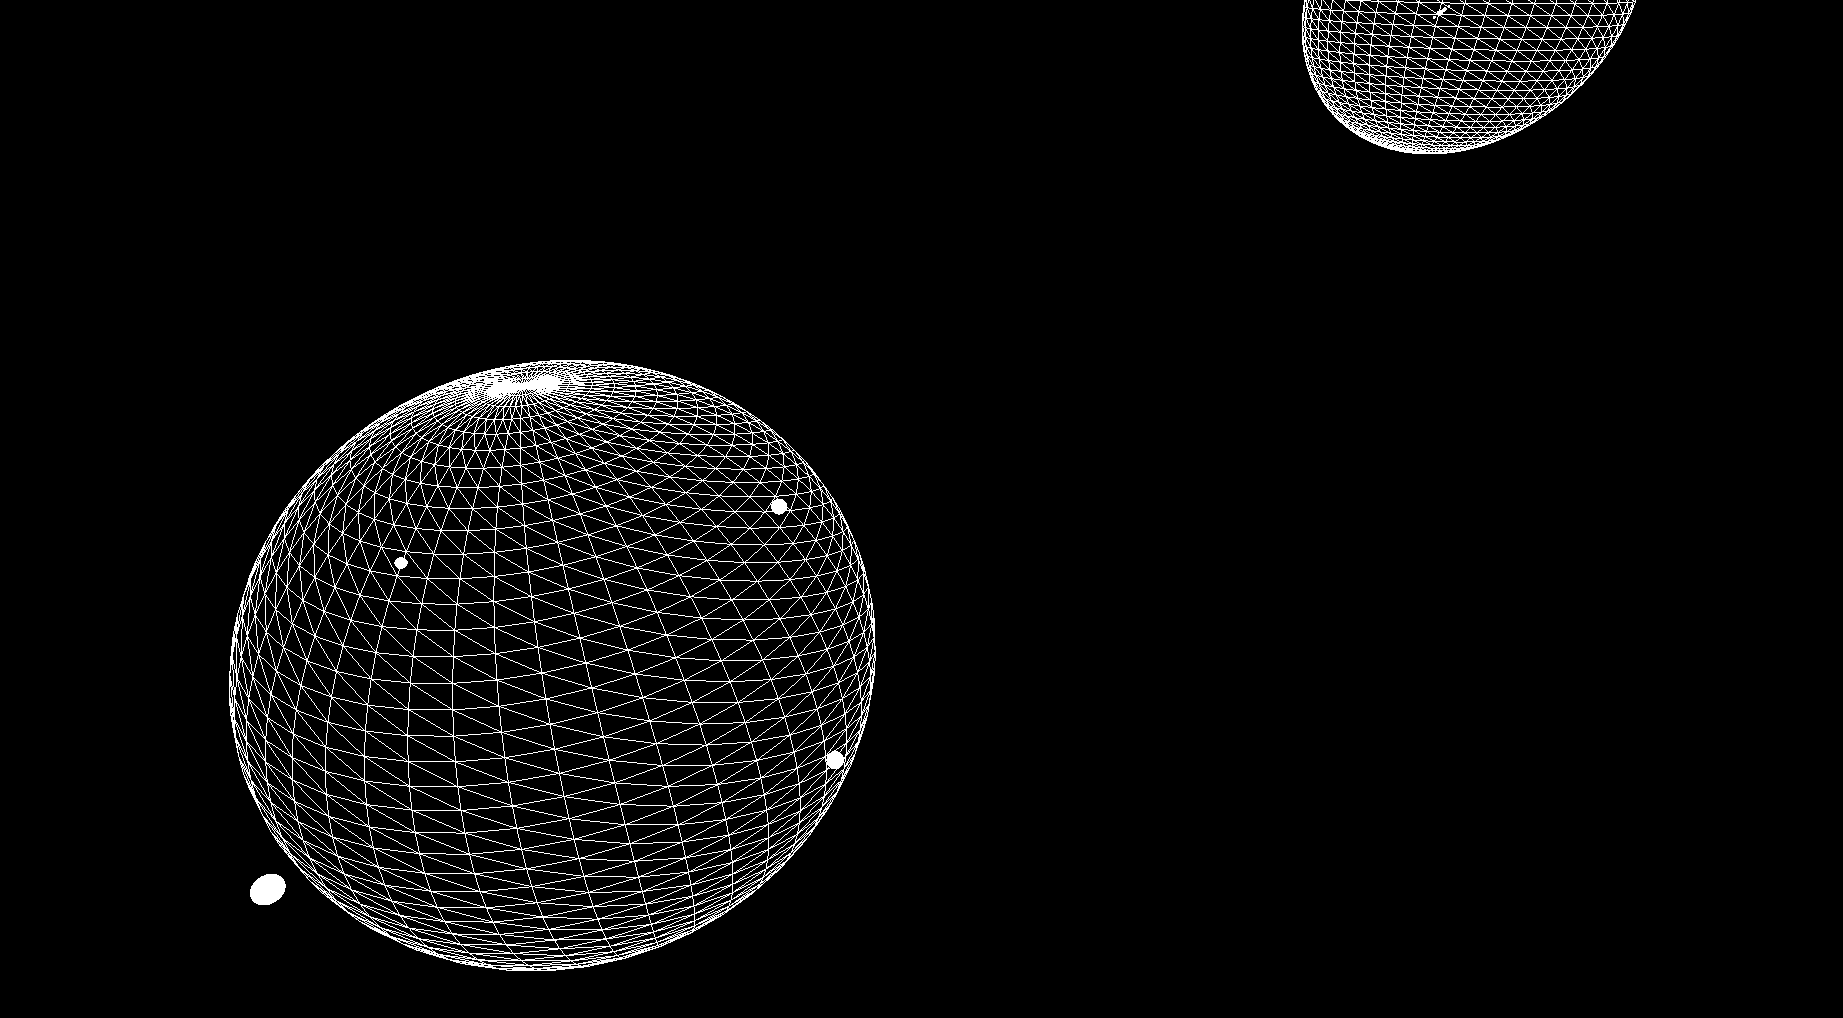
\includegraphics[width = 15cm,height = 10cm]{4.png}
\caption{\texttt{demo4}}
\label{fig:demo4}
\end{figure}

\begin{figure}[H]
\centering
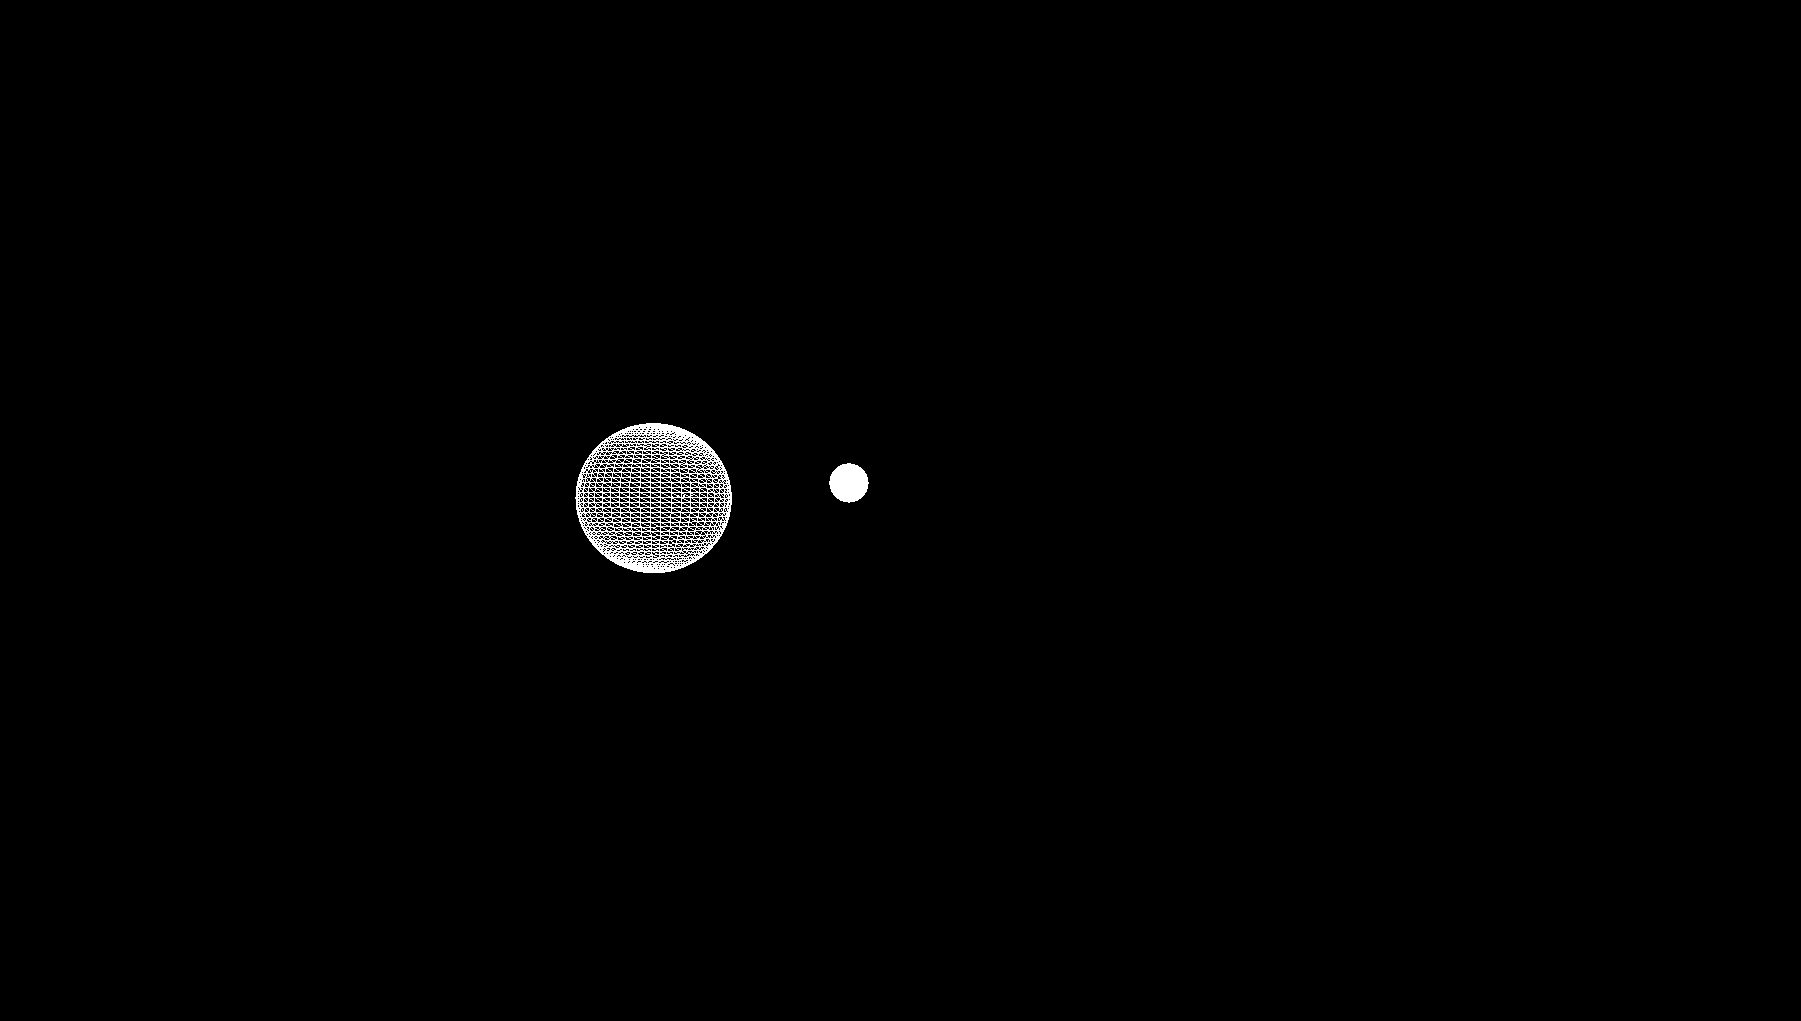
\includegraphics[width = 15cm,height = 10cm]{5.png}
\caption{\texttt{demo5}}
\label{fig:demo5}
\end{figure}

\begin{figure}[H]
\centering
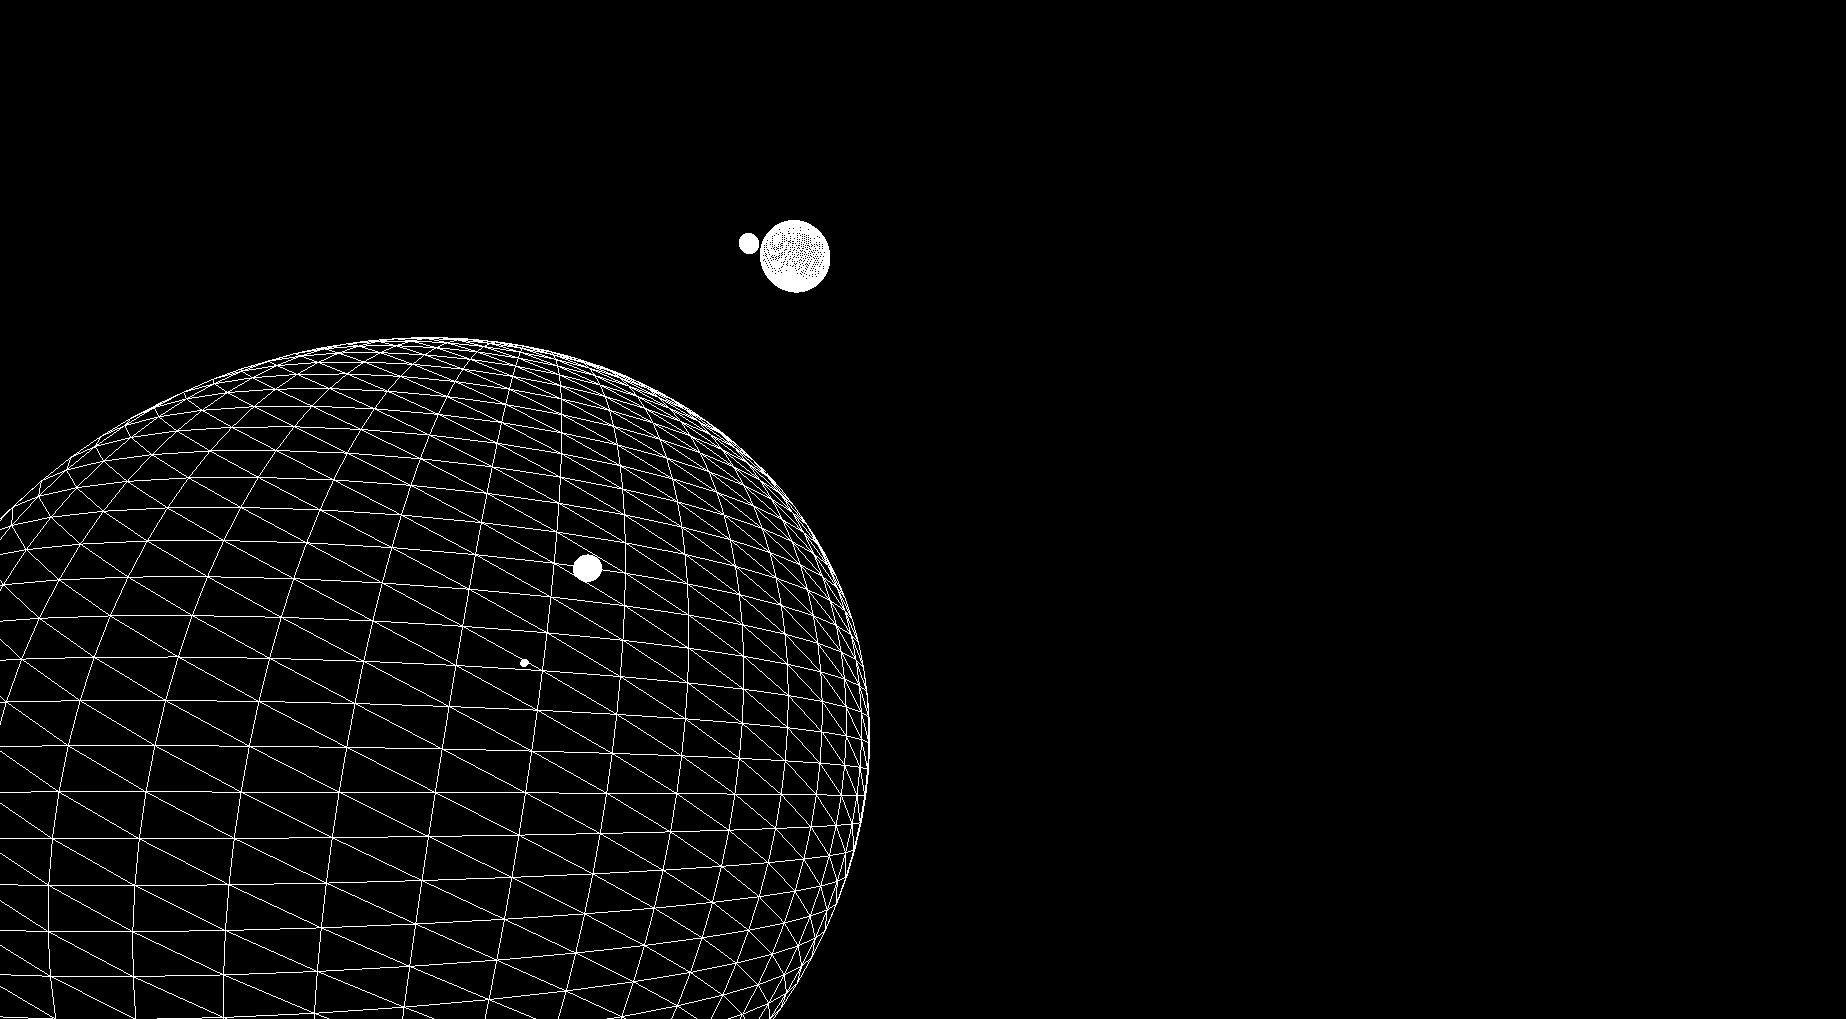
\includegraphics[width = 15cm,height = 10cm]{6.png}
\caption{\texttt{demo6}}
\label{fig:demo6}
\end{figure}

\begin{figure}[H]
\centering
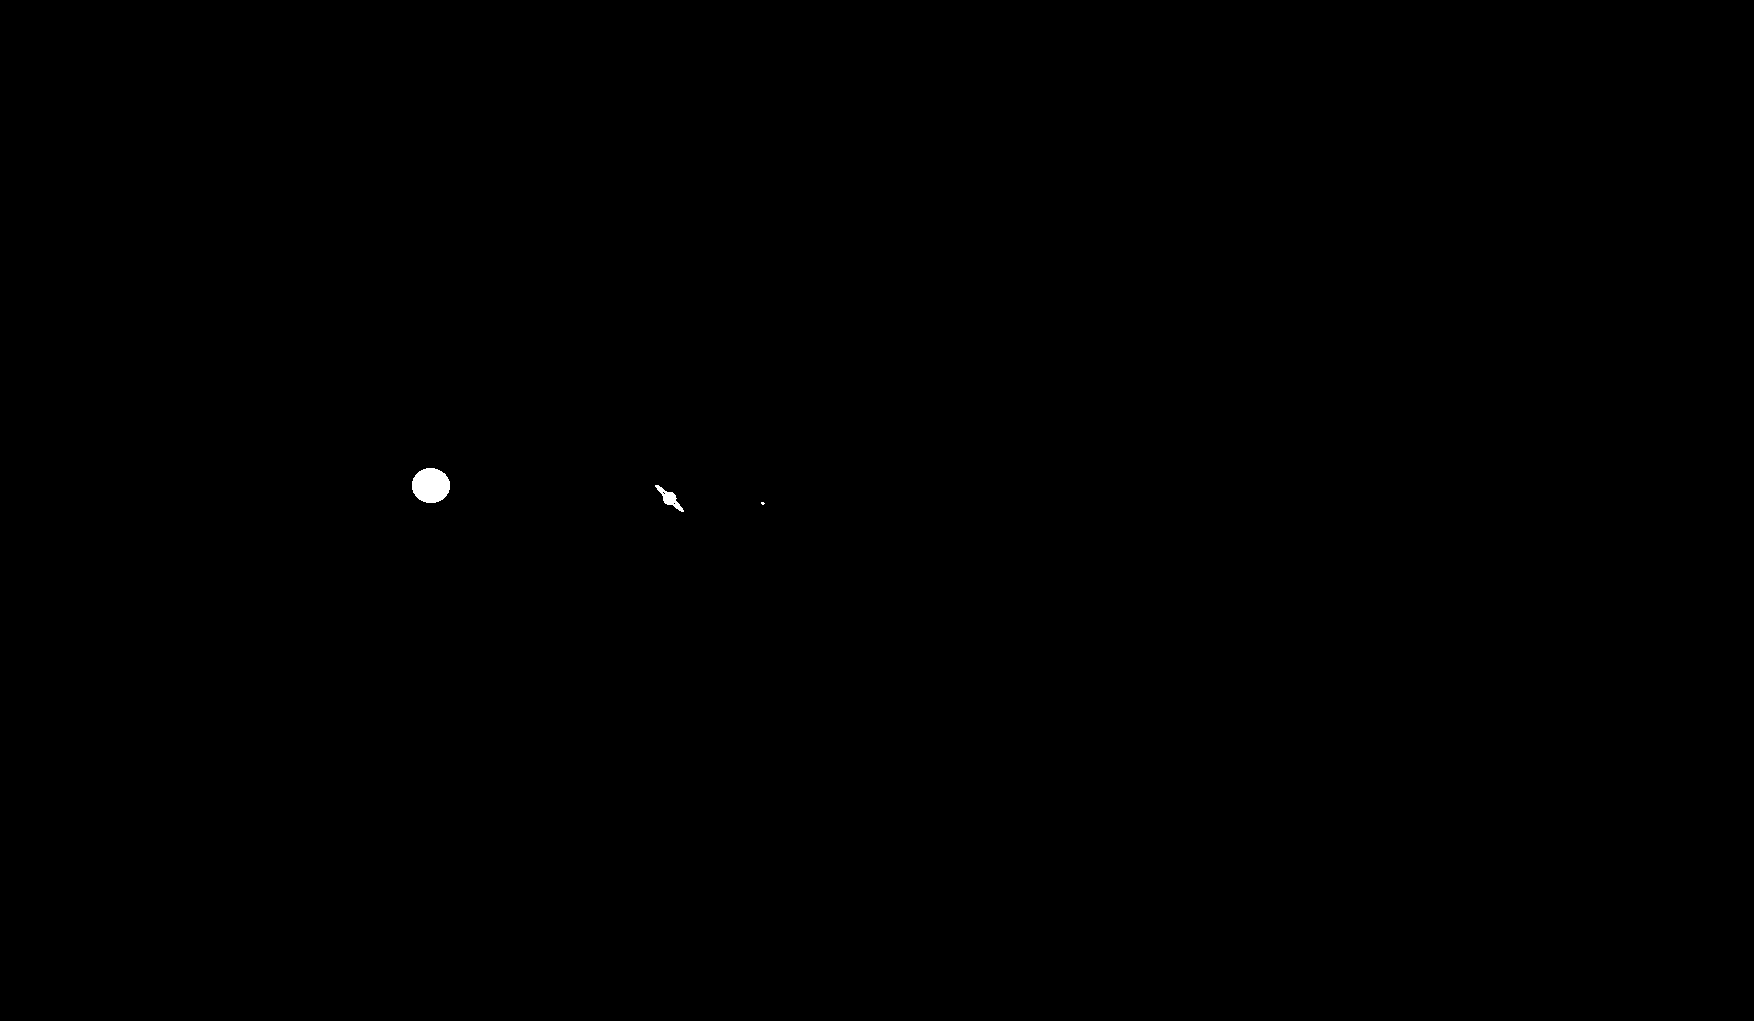
\includegraphics[width = 15cm,height = 10cm]{7.png}
\caption{\texttt{demo7}}
\label{fig:demo7}
\end{figure}



\newpage
\chapter{Conclusão}
A principal dificuldade enfrentada durante esta fase do trabalho foi a alteração da função que faz a leitura de ficheiros XML. A forma como o idealizamos o seu funcionamento não foi muito difícil, no entanto durante a sua implementação depara-mo-nos com alguns problemas de \textit{segmentation fault}, assim como transformações que ocorriam em locais inesperados. 

Um fator que também criou dificuldades foi a escolha de uma escalada adequada para definir o tamanho dos planetas e a distancia entre eles. Apesar de assim ser mais realista, não temos a certeza se foi a melhor opção.

Por ultimo, a alteração da câmara por forma a permitir "viajar" pelo sistema solar também não foi tarefa fácil e pensamos que a mesma ainda pode ser melhorada.

Contudo, apesar das dificuldades enfrentadas, podemos concluir que os objectivos foram atingidos.
\end{document}
